\section{Protocols}

\subsection{Master}

The master process is responsible for connecting to the coordinators, sending them configurations, and waiting for their final responses. Since it needs to complete only a linear sequence of steps, it runs in a single thread.

The master process begins by reading a configuration file with a list of IP addresses and ports at which coordinators can be reached. It opens a TCP connection with each of these and sends  configuration information about what agents the coordinator is responsible for at the start of the simulation, then waits for confirmations from all coordinators that the information was received (\texttt{CONFIG_CONFIRM}). It then waits for a second confirmation that all agents were launched successfully (\texttt{READY}) and the simulation can begin.

\begin{figure*}
    \begin{center}
        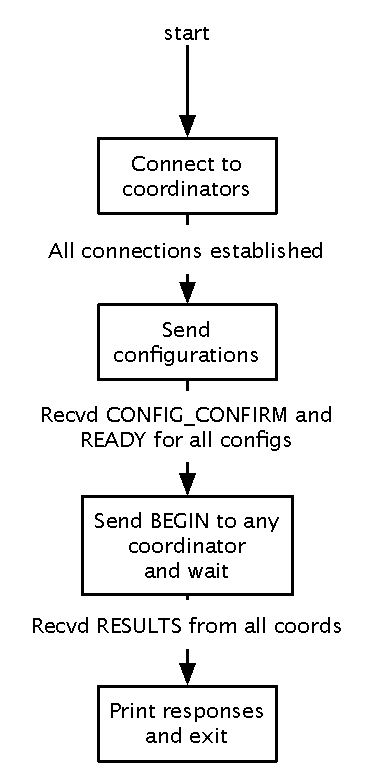
\includegraphics[scale=0.5]{figures/state_master.pdf}
    \end{center}
    \caption{State transition diagram for the master process.}
    \label{times}
\end{figure*}

